\documentclass[11pt]{article}

% ---------- packages ----------
\usepackage[utf8]{inputenc}
\usepackage[T1]{fontenc}
\usepackage{amsmath, amssymb, amsthm, mathrsfs}
\usepackage[margin=1in]{geometry}
\usepackage{enumitem}
\usepackage{xcolor}
\usepackage{tcolorbox}
\usepackage{tikz}
\usetikzlibrary{arrows.meta, positioning, calc}
\usepackage{pdflscape}
\usepackage{hyperref}
\hypersetup{colorlinks=true, linkcolor=blue!60!black, urlcolor=teal}

% ---------- theorem environments ----------
\theoremstyle{definition}
\newtheorem{definition}{Definition}[section]
\newtheorem{example}[definition]{Example}
\theoremstyle{plain}
\newtheorem{theorem}[definition]{Theorem}
\newtheorem{corollary}[definition]{Corollary}

% ---------- macros ----------
\newcommand{\R}{\mathbb{R}}
\newcommand{\C}{\mathbb{C}}
\newcommand{\N}{\mathbb{N}}
\newcommand{\Z}{\mathbb{Z}}
\newcommand{\CX}{\mathscr{C}}
\newcommand{\norm}[1]{\left\lVert #1 \right\rVert}
\newcommand{\abs}[1]{\left\lvert #1 \right\rvert}
\newcommand{\Gam}{\Gamma}
\renewcommand{\to}{\longrightarrow}

\title{\textbf{Rudin, \emph{Principles of Mathematical Analysis}}\\[4pt]
       Chapter 8 --- Some Special Functions\\[2pt]
       \large A High-Level Overview}
\author{}
\date{}

\begin{document}
\maketitle
\vspace{-2em}

\begin{abstract}
\noindent This is the \emph{payoff} chapter. Using the machinery of Chapter~7
(uniform convergence, the $M$-test, term-by-term differentiation, the
Stone--Weierstrass theorem), Rudin constructs and studies the most important
functions of analysis --- $e^x$, $\log x$, $\sin x$, $\cos x$, the number
$\pi$, and the gamma function $\Gamma$ --- entirely from \textbf{power series},
\emph{without} appealing to geometry. Along the way come Taylor's theorem, the
Fundamental Theorem of Algebra, Fourier series with Parseval's theorem, and
Stirling's formula.
\end{abstract}

% =====================================================================
% ----- Visual overview diagram (landscape) -----
\begin{landscape}
\thispagestyle{empty}
\vspace*{\fill}
\begin{center}
{\large\bfseries Visual Overview --- the logical skeleton of Chapter 8}\\[2pt]
{\itshape Build $\exp,\log,\sin,\cos,\pi,\Gamma$ rigorously from series --- no geometry assumed}\\[10pt]

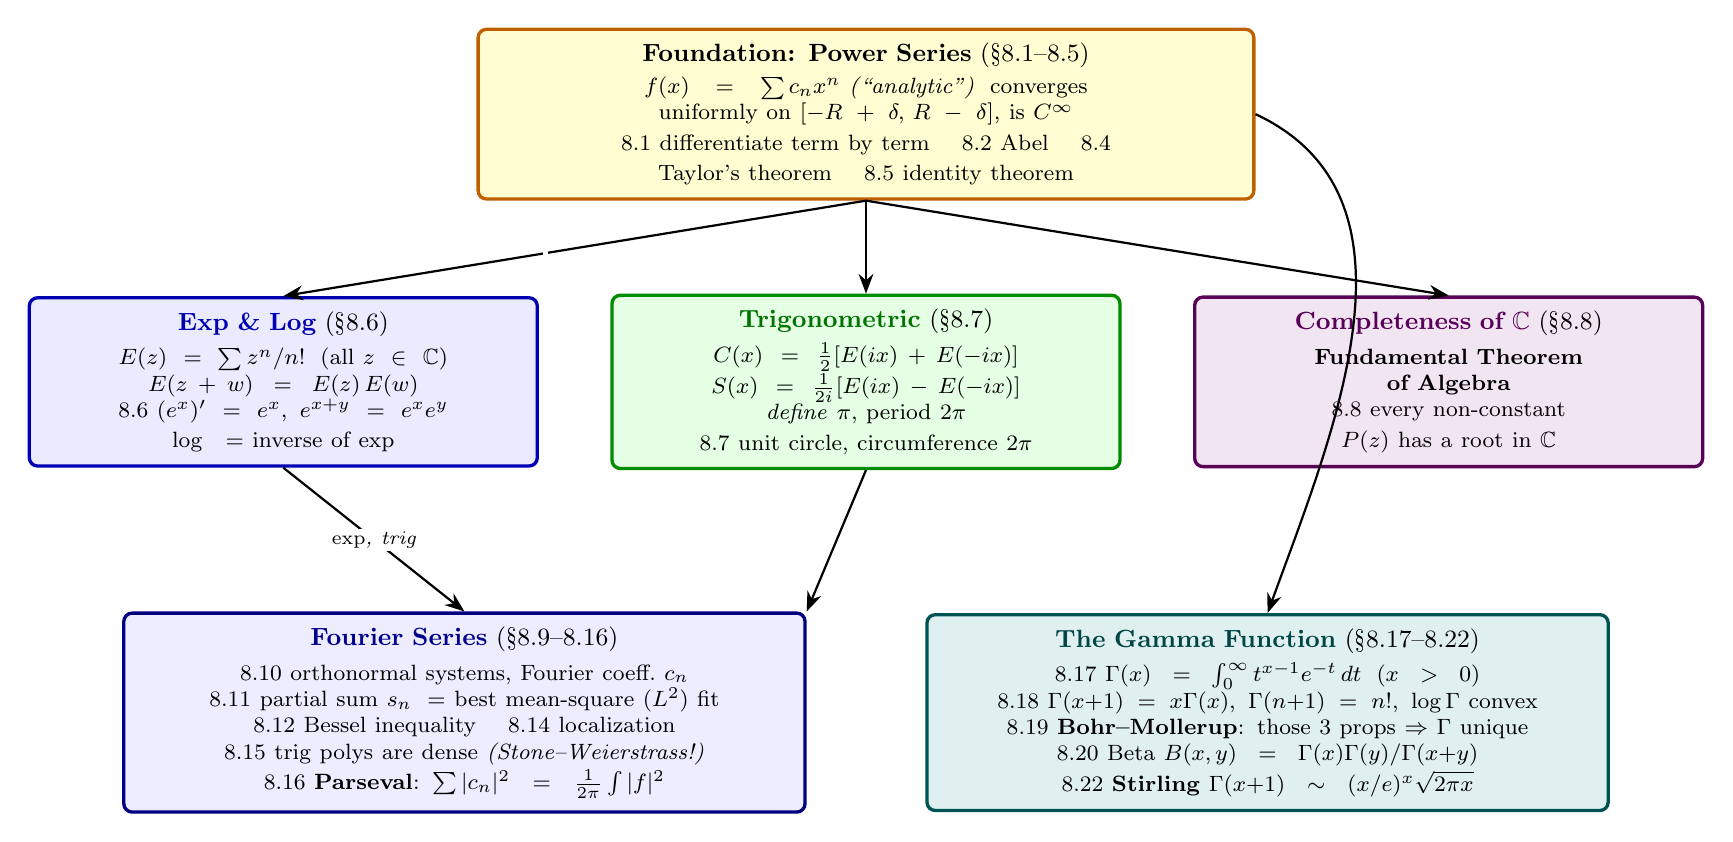
\begin{tikzpicture}[
   font=\small,
   >={Stealth[length=2.5mm]},
   box/.style={rounded corners=3pt, draw, very thick, align=center,
               inner sep=5pt, text width=#1},
   lbl/.style={font=\scriptsize\itshape, fill=white, inner sep=1pt},
]
% ---- foundation ----
\node[box=9.5cm, fill=yellow!18, draw=orange!75!black] (pow) at (0,0)
   {\textbf{Foundation: Power Series} (\S8.1--8.5)\\[2pt]
   \footnotesize
   $f(x)=\sum c_n x^n$ \emph{(``analytic'')} \;converges uniformly on $[-R+\delta,\,R-\delta]$, is $C^\infty$\\
   8.1 differentiate term by term \quad 8.2 Abel \quad 8.4 Taylor's theorem \quad 8.5 identity theorem};

% ---- three constructed families ----
\node[box=6.1cm, fill=blue!8, draw=blue!70!black] (exp) at (-7.4,-3.4)
   {\textbf{\textcolor{blue!70!black}{Exp \& Log}} (\S8.6)\\[3pt]
   \footnotesize
   $E(z)=\sum z^n/n!$ \;(all $z\in\C$)\\
   $E(z+w)=E(z)\,E(w)$\\
   8.6 $(e^x)'=e^x,\ e^{x+y}=e^xe^y$\\
   $\log=$ inverse of $\exp$};

\node[box=6.1cm, fill=green!10, draw=green!55!black] (trig) at (0,-3.4)
   {\textbf{\textcolor{green!45!black}{Trigonometric}} (\S8.7)\\[3pt]
   \footnotesize
   $C(x)=\tfrac12[E(ix)+E(-ix)]$\\
   $S(x)=\tfrac1{2i}[E(ix)-E(-ix)]$\\
   \emph{define} $\pi$, period $2\pi$\\
   8.7 unit circle, circumference $2\pi$};

\node[box=6.1cm, fill=violet!10, draw=violet!70!black] (fta) at (7.4,-3.4)
   {\textbf{\textcolor{violet!70!black}{Completeness of $\C$}} (\S8.8)\\[3pt]
   \footnotesize
   \textbf{Fundamental Theorem}\\
   \textbf{of Algebra}\\
   8.8 every non-constant\\
   $P(z)$ has a root in $\C$};

% ---- two deep applications ----
\node[box=8.3cm, fill=blue!7!white, draw=blue!50!black] (four) at (-5.1,-7.6)
   {\textbf{\textcolor{blue!55!black}{Fourier Series}} (\S8.9--8.16)\\[3pt]
   \footnotesize
   8.10 orthonormal systems, Fourier coeff.\ $c_n$\\
   8.11 partial sum $s_n=$ best mean-square ($L^2$) fit\\
   8.12 Bessel inequality \quad 8.14 localization\\
   8.15 trig polys are dense \emph{(Stone--Weierstrass!)}\\
   8.16 \textbf{Parseval}: $\sum|c_n|^2=\frac{1}{2\pi}\int|f|^2$};

\node[box=8.3cm, fill=teal!12, draw=teal!65!black] (gam) at (5.1,-7.6)
   {\textbf{\textcolor{teal!55!black}{The Gamma Function}} (\S8.17--8.22)\\[3pt]
   \footnotesize
   8.17 $\Gamma(x)=\int_0^\infty t^{x-1}e^{-t}\,dt$ \;($x>0$)\\
   8.18 $\Gamma(x{+}1)=x\Gamma(x),\ \Gamma(n{+}1)=n!,\ \log\Gamma$ convex\\
   8.19 \textbf{Bohr--Mollerup}: those 3 props $\Rightarrow$ $\Gamma$ unique\\
   8.20 Beta $B(x,y)=\Gamma(x)\Gamma(y)/\Gamma(x{+}y)$\\
   8.22 \textbf{Stirling} $\Gamma(x{+}1)\sim(x/e)^x\sqrt{2\pi x}$};

% ---- arrows ----
\draw[->, thick] (pow.south) -- (exp.north)  node[lbl,pos=0.55]{};
\draw[->, thick] (pow.south) -- (trig.north);
\draw[->, thick] (pow.south) -- (fta.north);
\draw[->, thick] (exp.south) -- (four.north) node[lbl,pos=0.5]{$\exp$, trig};
\draw[->, thick] (trig.south) -- (four.north east);
\draw[->, thick] (pow.east) to[out=-25,in=70] (gam.north);
\end{tikzpicture}

\vspace{6pt}
{\footnotesize Book pp.\ 172--203 \;\textbullet\; uses the Chapter~7 engine: uniform convergence, $M$-test, Stone--Weierstrass.}
\end{center}
\vspace*{\fill}
\end{landscape}

% =====================================================================
\section{Power Series --- the Foundation (\S8.1--8.5)}

\begin{definition}[Analytic function]
A function represented by a power series
\[
   f(x)=\sum_{n=0}^{\infty} c_n x^n,
   \qquad\text{or more generally}\qquad
   f(x)=\sum_{n=0}^{\infty} c_n (x-a)^n,
\]
is called \emph{analytic}. If the first series converges on $(-R,R)$ we say
$f$ is expanded about $0$; here $R$ is the radius (interval) of convergence.
\end{definition}

\begin{theorem}[Term-by-term differentiation, 8.1]
If $f(x)=\sum c_n x^n$ converges for $\abs{x}<R$, then the series converges
\emph{uniformly} on $[-R+\delta,\,R-\delta]$ for every $\delta>0$; $f$ is
continuous and differentiable on $(-R,R)$, and
\[
   f'(x)=\sum_{n=1}^{\infty} n\,c_n x^{n-1}.
\]
\end{theorem}

\begin{corollary}
$f$ has derivatives of \emph{all} orders on $(-R,R)$, given by repeated
term-by-term differentiation, and $c_n = f^{(n)}(0)/n!$.
\end{corollary}

\begin{theorem}[Abel, 8.2]
If $\sum c_n$ converges and $f(x)=\sum c_n x^n$ for $\abs{x}<1$, then
$\displaystyle\lim_{x\to 1^-} f(x)=\sum_{n=0}^{\infty} c_n$.
\end{theorem}

\begin{theorem}[Taylor's theorem, 8.4]
If $f(x)=\sum c_n x^n$ converges on $\abs{x}<R$ and $-R<a<R$, then $f$ can be
re-expanded about $a$:
\[
   f(x)=\sum_{n=0}^{\infty}\frac{f^{(n)}(a)}{n!}(x-a)^n
   \qquad (\abs{x-a}<R-\abs{a}).
\]
\end{theorem}

\begin{theorem}[Identity theorem, 8.5]
If $\sum a_n x^n=\sum b_n x^n$ on a set with a limit point in $(-R,R)$, then
$a_n=b_n$ for all $n$. (A power series is determined by its values near any point.)
\end{theorem}

% =====================================================================
\section{The Exponential and Logarithmic Functions (\S8.6)}

\begin{definition}[The exponential]
For every complex $z$,
\[
   E(z)=\sum_{n=0}^{\infty}\frac{z^n}{n!}
   \qquad(\text{converges for all }z\in\C\text{ by the ratio test}).
\]
Multiplying absolutely convergent series gives the \textbf{addition formula}
\[
   E(z)\,E(w)=\sum_{n=0}^{\infty}\frac{(z+w)^n}{n!}=E(z+w).
\]
\end{definition}

\begin{theorem}[Properties of $e^x$, 8.6]
With $e^x:=E(x)$ on $\R$:
\begin{enumerate}[label=(\alph*), leftmargin=2em, itemsep=0pt]
  \item $e^x$ is continuous and differentiable, with $(e^x)'=e^x$;
  \item $e^x$ is strictly increasing and $e^x>0$;
  \item $e^{x+y}=e^x e^y$;
  \item $e^x\to+\infty$ as $x\to+\infty$, \; $e^x\to 0$ as $x\to-\infty$;
  \item $\displaystyle\lim_{x\to+\infty} x^n e^{-x}=0$ for every $n$ ($e^x$ beats every power).
\end{enumerate}
Since $E$ is strictly increasing and differentiable, it has an inverse $L=\log$,
also strictly increasing and differentiable, defined on $(0,\infty)$.
\end{theorem}

% =====================================================================
\section{The Trigonometric Functions (\S8.7)}

\begin{definition}[Cosine and sine, from $E$]
\[
   C(x)=\tfrac12\!\left[E(ix)+E(-ix)\right],
   \qquad
   S(x)=\tfrac1{2i}\!\left[E(ix)-E(-ix)\right],
\]
so that $E(ix)=C(x)+iS(x)$, $\;\abs{E(ix)}=1$, $\;C'=-S$, $\;S'=C$, and
$C^2+S^2=1$. These coincide with $\cos x$ and $\sin x$ --- but defined
analytically, with no geometry.
\end{definition}

\begin{theorem}[Periodicity and $\pi$, 8.7]
Define $\pi$ so that $\pi/2$ is the smallest positive zero of $C$. Then
\begin{enumerate}[label=(\alph*), leftmargin=2em, itemsep=0pt]
  \item $E$ is periodic with period $2\pi i$;
  \item $C$ and $S$ are periodic with period $2\pi$;
  \item if $0<t<2\pi$ then $E(it)\neq 1$;
  \item every $z\in\C$ with $\abs{z}=1$ equals $E(it)$ for a unique $t\in[0,2\pi)$.
\end{enumerate}
Consequently $\gamma(t)=E(it)$, $0\le t\le 2\pi$, is a simple closed curve
tracing the unit circle, of length $\int_0^{2\pi}\abs{\gamma'(t)}\,dt=2\pi$ ---
giving $\pi$ its usual geometric meaning.
\end{theorem}

% =====================================================================
\section{Algebraic Completeness of $\C$ (\S8.8)}

\begin{theorem}[Fundamental Theorem of Algebra, 8.8]
If $a_0,\dots,a_n\in\C$ with $n\ge 1$ and $a_n\neq 0$, and
$P(z)=\sum_{k=0}^{n} a_k z^k$, then $P(z)=0$ for some $z\in\C$.
\end{theorem}

\noindent\emph{Idea of proof.} Let $\mu=\inf_{z}\abs{P(z)}$. Since
$\abs{P(z)}\to\infty$ as $\abs{z}\to\infty$, the infimum is attained at some
$z_0$. If $P(z_0)\neq 0$ one can perturb $z_0$ to \emph{decrease} $\abs{P}$
(using $E(it)$ to choose a direction), contradicting minimality. Hence
$P(z_0)=0$: every non-constant complex polynomial has a root, so $\C$ is
algebraically closed.

% =====================================================================
\section{Fourier Series (\S8.9--8.16)}

\begin{definition}[Trigonometric polynomial / orthonormal system, 8.9--8.10]
A \emph{trigonometric polynomial} is $f(x)=a_0+\sum_{n=1}^{N}(a_n\cos nx+b_n\sin nx)$.
A sequence $\{\phi_n\}$ is \emph{orthonormal} on $[a,b]$ if
$\int_a^b \phi_n\overline{\phi_m}\,dx=\delta_{nm}$; e.g.\ $\{(2\pi)^{-1/2}e^{inx}\}$
on $[-\pi,\pi]$. The \emph{Fourier coefficients} of $f$ are
$c_n=\int_a^b f\,\overline{\phi_n}\,dx$.
\end{definition}

\begin{theorem}[Best mean-square approximation, 8.11]
Among all $t_n=\sum_{m=1}^{n}\gamma_m\phi_m$, the partial Fourier sum
$s_n=\sum_{m=1}^{n} c_m\phi_m$ minimizes $\int_a^b\abs{f-t_n}^2\,dx$; minimum is
attained \emph{iff} $\gamma_m=c_m$. (Fourier partial sums are the orthogonal
projection onto the span of $\phi_1,\dots,\phi_n$.)
\end{theorem}

\begin{theorem}[Bessel inequality (8.12) \& localization (8.14)]
$\displaystyle\sum_{n=1}^{\infty}\abs{c_n}^2\le\int_a^b\abs{f}^2\,dx$, so $c_n\to 0$.
Moreover if $f$ satisfies a Lipschitz-type bound near $x$
($\abs{f(x+t)-f(x)}\le M\abs{t}$), then $s_N(f;x)\to f(x)$: convergence at a
point depends only on the \emph{local} behaviour of $f$.
\end{theorem}

\begin{theorem}[Density (8.15) \& Parseval (8.16)]
If $f$ is continuous with period $2\pi$, then for every $\varepsilon>0$ there is
a trigonometric polynomial $P$ with $\abs{f(x)-P(x)}<\varepsilon$ for all $x$
(a corollary of Stone--Weierstrass). Consequently, for Riemann-integrable
$2\pi$-periodic $f\sim\sum c_n e^{inx}$,
\[
   \frac{1}{2\pi}\int_{-\pi}^{\pi}\abs{f(x)}^2\,dx
   =\sum_{n=-\infty}^{\infty}\abs{c_n}^2
   \qquad\textbf{(Parseval).}
\]
\end{theorem}

% =====================================================================
\section{The Gamma Function (\S8.17--8.22)}

\begin{definition}[Gamma, 8.17]
For $0<x<\infty$,
\[
   \Gam(x)=\int_0^{\infty} t^{x-1}e^{-t}\,dt
   \qquad(\text{the integral converges}).
\]
\end{definition}

\begin{theorem}[Functional equation, 8.18]
On $(0,\infty)$:
\textbf{(a)} $\Gam(x+1)=x\,\Gam(x)$ (integration by parts);
\textbf{(b)} $\Gam(n+1)=n!$ for $n\in\N$ (so $\Gam$ interpolates the factorial);
\textbf{(c)} $\log\Gam$ is convex.
\end{theorem}

\begin{theorem}[Bohr--Mollerup characterization, 8.19]
If $f>0$ on $(0,\infty)$ satisfies $f(x+1)=xf(x)$, $f(1)=1$, and $\log f$ is
convex, then $f=\Gam$. \emph{These three properties pin $\Gam$ down uniquely}; a
by-product is
$\displaystyle\Gam(x)=\lim_{n\to\infty}\frac{n!\,n^x}{x(x+1)\cdots(x+n)}$.
\end{theorem}

\begin{theorem}[Beta function (8.20) \& Stirling (8.22)]
For $x,y>0$,
\[
   B(x,y)=\int_0^1 t^{x-1}(1-t)^{y-1}\,dt=\frac{\Gam(x)\,\Gam(y)}{\Gam(x+y)} .
\]
And for large $x$ (hence large $n!$), \textbf{Stirling's formula}:
\[
   \lim_{x\to\infty}\frac{\Gam(x+1)}{(x/e)^x\sqrt{2\pi x}}=1 .
\]
\end{theorem}

% =====================================================================
\section*{The big picture}
\addcontentsline{toc}{section}{The big picture}
Chapter 8 \emph{cashes in} Chapter 7. Power series (made legitimate by uniform
convergence) define $\exp$; from $\exp$ come $\log$, $\sin$, $\cos$, and $\pi$;
the same circle group $E(it)$ proves the Fundamental Theorem of Algebra. Two
deeper applications follow: Fourier series (where Stone--Weierstrass guarantees
trigonometric approximation and Parseval gives an $L^2$ isometry) and the gamma
function (the factorial extended to all real --- and complex --- arguments,
characterized by Bohr--Mollerup and estimated by Stirling).

\end{document}
